\chapter{Attending to Remember: Recent Advances in Methods and Theory}\label{ch:attending-to-remember}

Hallmarks of human cognition, such as forming and carrying out complex plans in pursuit of goals or flexibly engaging in intricate and dynamic social interactions, are supported in part by an ensemble of neurocognitive mechanisms that enable episodic memory—that is, the ability to learn and later bring back to mind details from past experiences. Although much progress has been made in understanding episodic memory, there remain open questions about some of the key mechanisms that impact remembering or forgetting in any given moment. Attention, in particular, is one set of processes implicated in learning and remembering since the earliest investigations into episodic memory \parencite{ebbinghaus1885memory}. Over the ensuing decades, remarkable advances have been made in understanding multiple forms of attention and how attention mechanisms modulate learning and lead to variability in whether and how we remember. Here, we highlight recent methodological advances and concomitant theoretical insights into how attention impacts learning and remembering and note important open questions and promising future directions.

\section{Interactions Between Neural Networks of Attention, Goal-State Processes, and Memory}

Cognitive scientists and neuroscientists have made tremendous progress in specifying and measuring different forms of attention, their neural mechanisms, as well as their interactions with related cognitive control processes. A central insight is the dichotomous nature of attention. Namely, there is top-down (goal-directed or endogenous) orienting of attention to and selection of goal-relevant stimuli, which contrasts with bottom-up (stimulus-driven or exogenous) attentional capture \parencite[e.g.,][]{corbetta2002control,posner1990attention}. To illustrate, consider this real-world driving scenario: While preparing to turn onto a specific street, top-down selective attention is directed toward street-name signs, whereas bottom-up attentional capture is prompted by the unexpected event of a dog running out from between two parked cars. Top-down and bottom-up attention systems dynamically interact with related mechanisms of cognitive control, including those that subserve the representation of goals and enable goals to govern attention and information processing. The interactions between attention and cognitive control are bidirectional: Not only do goal states influence attention, but attention also impacts goal representation.

As depicted in Figure~\ref{fig:a2r-fig1}a, there are three frontoparietal networks central to attention and cognitive control: top-down attention via the dorsal attention network, bottom-up attention via the ventral attention network, and the cognitive control network \parencite[also known as the frontoparietal control network;][]{cole2007cognitive,corbetta2002control,corbetta2008reorienting,menon2022role}. With respect to episodic memory, attention and cognitive control mechanisms can affect the representations of perceived and retrieved event features in the neocortex along with memory-relevant computations and representations within the medial temporal lobe \parencite[e.g.,][]{cabeza2008parietal,dobbins2005domain,hutchinson2014functional,uncapher2009posterior}. Both the intensity of attention as well as its selectivity are at least two ways in which attention impacts memory encoding and retrieval.

\begin{figure}[!tbp]
	\centering
	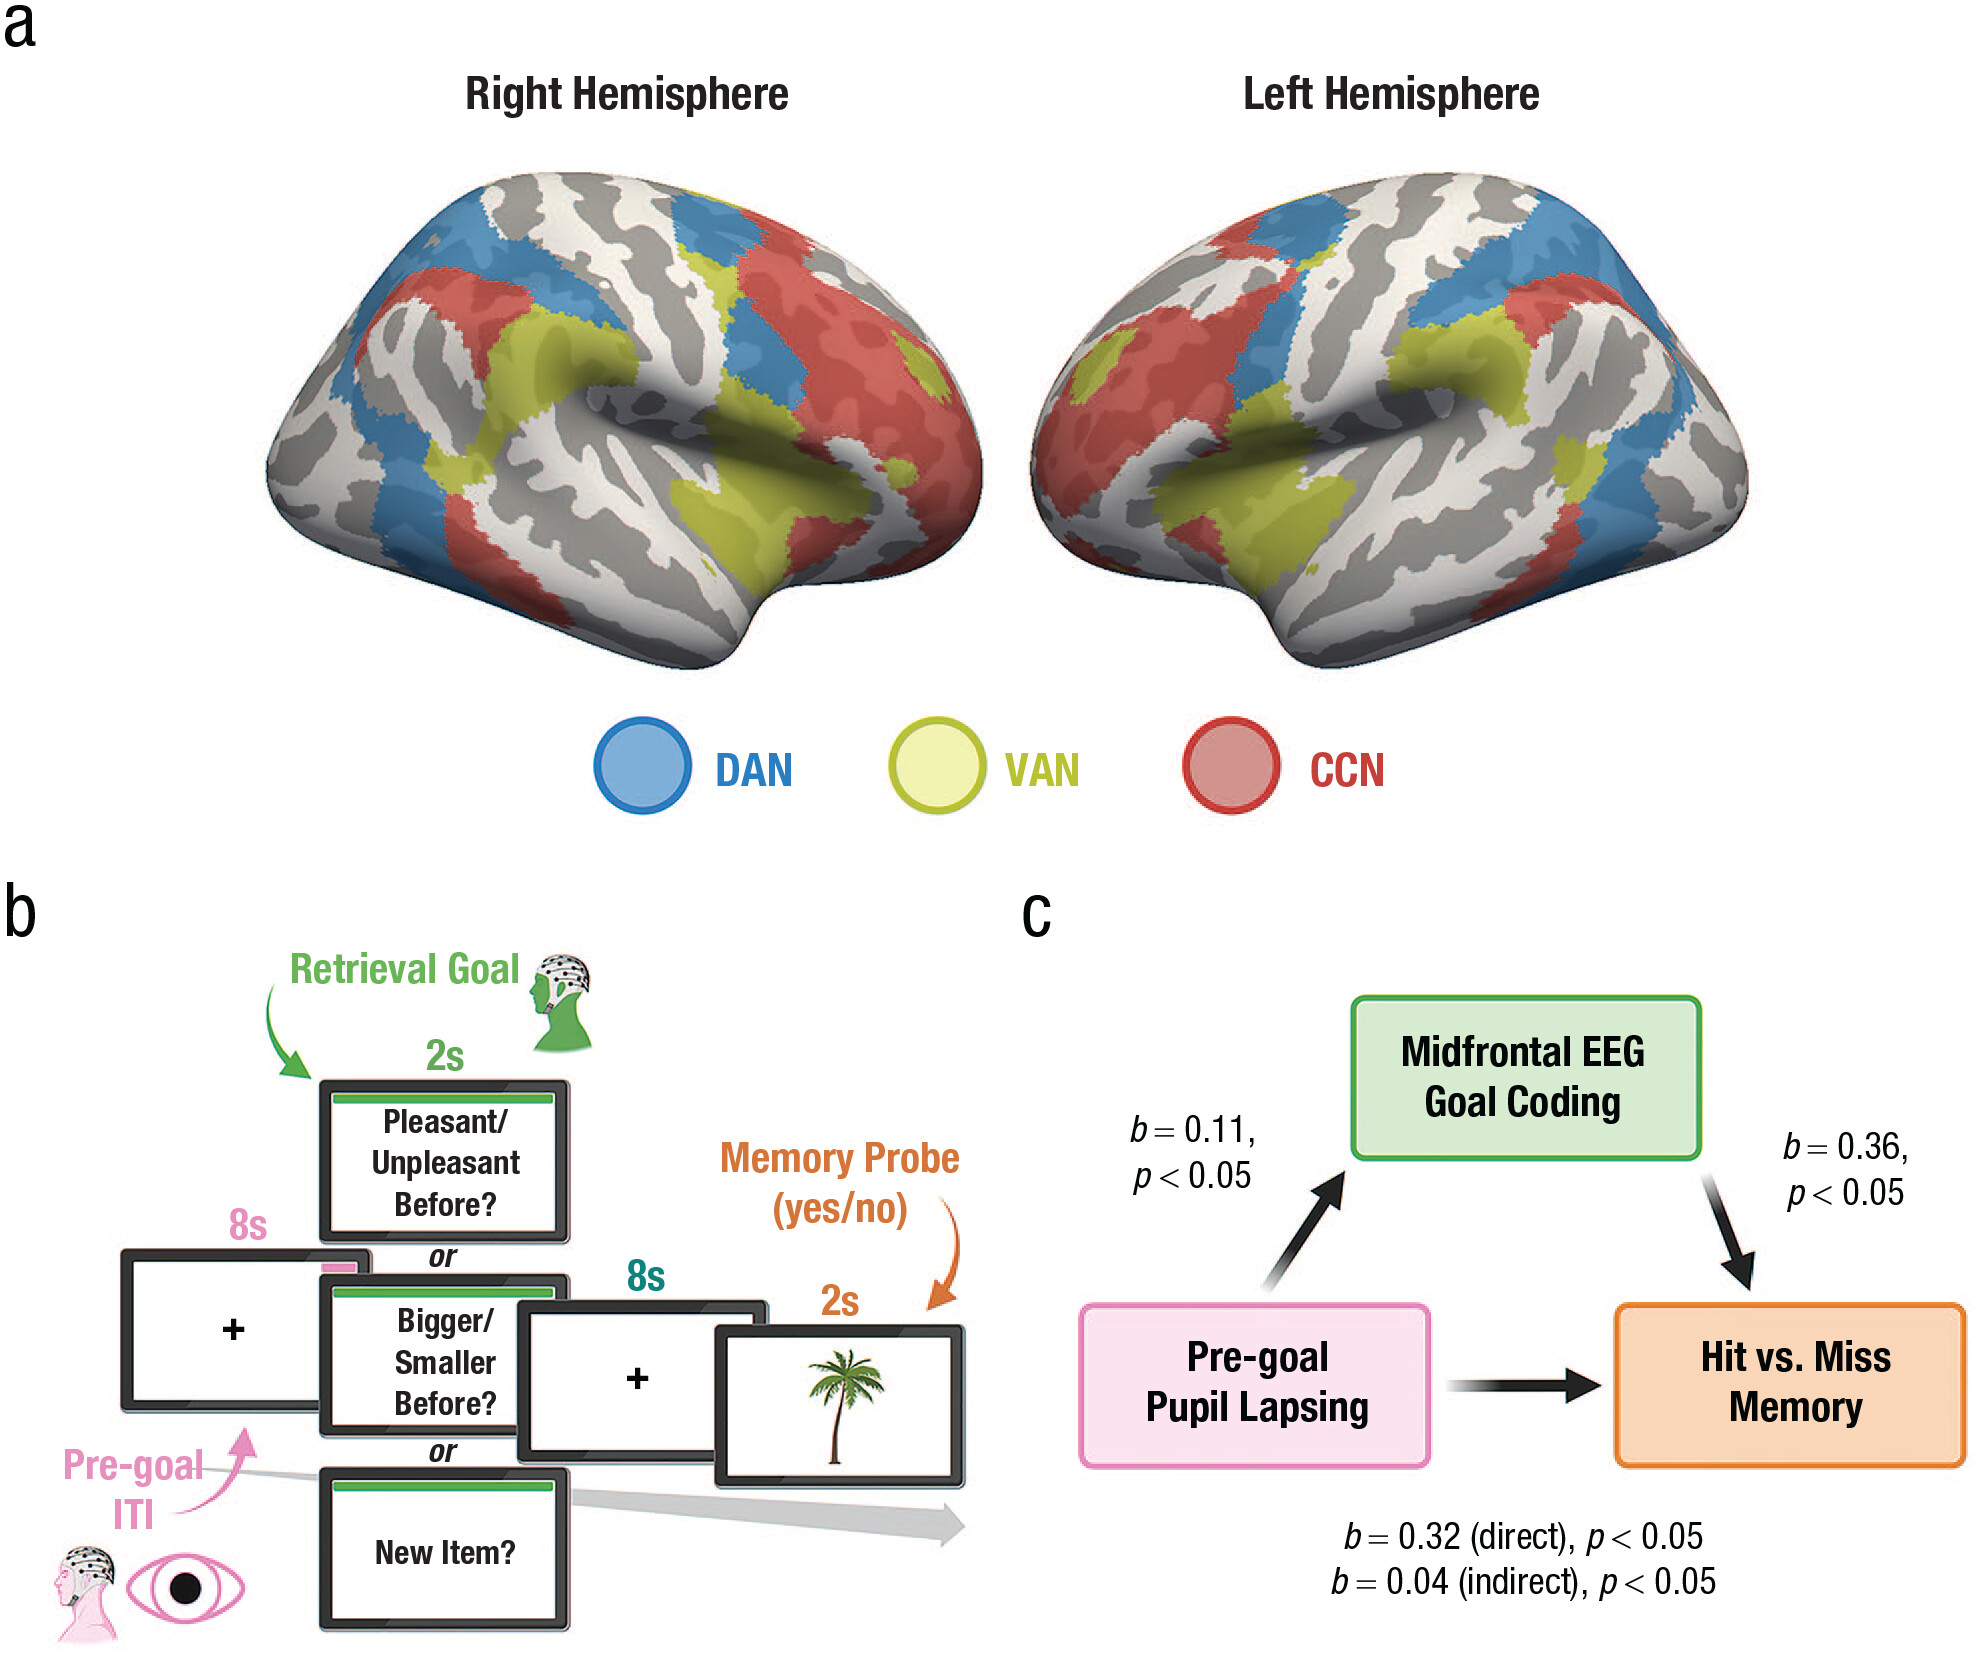
\includegraphics[width=1\linewidth]{figures/attending_to_remember-fig1.jpg}
	\caption[Assessing the influence of attention on memory retrieval]{Assessing the influence of attention on memory retrieval. Shown in (a) are the frontoparietal networks of attention and cognitive control derived from network parcellations computed from the full sample (\textit{N} = 1,000) in \textcite{yeo2011organization}. The schematic of the goal-directed memory-retrieval task used in \textcite{madore2020memory} shows (b) that pre-goal lapsing was measured using EEG posterior alpha power and pupil size in the last 1 s of the ITI, whereas goal-coding strength was measured using a retrieval goal-cue-locked ERP extracted from a midfrontal cluster of electrodes. In (c) the 1 s prior to the onset of the retrieval goal cue, pupil size (and posterior alpha power; not shown) significantly correlated with retrieval success, and midfrontal EEG goal-coding strength partially mediated this effect \parencite[\textit{n} = 75;][]{madore2020memory}. DAN = dorsal attention network; VAN = ventral attention network; CCN = cognitive control network; ITI = intertrial interval; ERP = event-related potential. Created in BioRender \parencite{schwartz2025a}. \url{https://BioRender.com/mejp1fu}.}
	\label{fig:a2r-fig1}
\end{figure}
\FloatBarrier

New insights into interactions between attention, cognitive control, and memory have come from studies leveraging readouts of attention and/or goal states during the acquisition and expression of episodic memories. This includes utilizing temporally resolved psychophysiological tools—such as reaction-time variability, pupil diameter, and posterior alpha (8–12 Hz) power (see Table~\ref{tab:glossary}) assayed via scalp EEG—to measure moment-to-moment attentional fluctuations and between-individuals attentional variability. Adopting these tools, multiple studies have revealed that the strength of top-down attention just prior to and during learning or an attempt to remember correlates with memory performance \parencite[i.e., readiness to learn and readiness to remember; e.g.,][]{cohen2015peri,madore2020memory,madore2022readiness,miller2020variation,miller2019individual,robison2022pupillary}.

\begin{table}[ht!]
	\captionsetup{justification=raggedright,singlelinecheck=off}
	\caption{Glossary}
	\label{tab:glossary}
	\noindent\rule{\linewidth}{0.4pt}
	\begin{itemize}
		\item \textbf{Posterior alpha (8--12 Hz) power:} A quantity derived from a cluster of posterior scalp EEG electrodes (over the occipital and parietal cortex) representing the squared amplitude of sinusoidal components typically within the frequency range between 8 and 12 Hz. Decreases in alpha power are often associated with engagement of top-down attention.
		\item \textbf{Pattern-classification methods:} Machine-learning-based approaches in which a classifier is trained to differentiate the patterns of brain activity associated with two or more experimental conditions and/or behavioral outcomes. The classifier is tested on independent brain patterns from held-out trials after training and can be used to quantify the strength of pattern evidence on any given test trial. For functional MRI (fMRI), the patterns used for training and tests constitute a vector of voxels from a brain region; when applied to fMRI data, this method is often referred to as multivoxel pattern analysis.
		\item \textbf{Event-based feature representation:} Neural pattern of activity elicited by an encountered stimulus or event and thought to code for an aspect (feature) of the event. The strength or fidelity of an event-based feature representation can be quantified with pattern-classification methods.
		\item \textbf{Neocortical structural variability:} Interindividual differences in brain morphology in the neocortex. One example is differences in gray matter volume (which relates to structural integrity) in a particular neocortical region.
		\item \textbf{Closed-loop interface:} Self-regulating system in which the output controls the input, which in turn controls the output (e.g., a thermostat).
	\end{itemize}
	\noindent\rule{\linewidth}{0.4pt}
\end{table}

To illustrate, one recent experiment examined interactions between attention, goal coding, and memory using a goal-directed associative memory task in which during each retrieval trial (Fig.~\ref{fig:a2r-fig1}b) participants were asked to indicate whether they remembered a test probe as having been previously encountered in one of two task contexts during an immediately preceding study phase. \footnote{During the memory encoding (study) phase, participants encountered images of everyday objects that were physically small (e.g., fixed at 150 × 150 pixels) or large (e.g., fixed at 450 × 450 pixels) on the screen on any given trial. Some of the objects were normatively more pleasant than others. On half of the study trials, participants were instructed to decide whether the upcoming object would be physically small or large; on the other half of trials, participants were instructed to indicate whether the upcoming object would be pleasant or unpleasant.} During the retrieval phase, participants were cued with one of three retrieval goals on any given trial. Readouts of top-down attention just prior to goal cueing included pupil size and EEG posterior alpha power, and the strength of goal coding was measured via a midfrontal event-related potential elicited by the retrieval goal cue.\footnote{An alternative approach to measuring the strength of goal representations is to use pattern-classification methods to quantify the strength of goal representation using neural-activity patterns within the frontoparietal control network \parencite[e.g.,][]{waskom2014frontoparietal}.} Analyses revealed that goal-coding strength varied as a function of the level of attention evident in the moment just prior to retrieval goal onset and that these interactions between attention and goal coding predicted whether retrieval would be successful or unsuccessful \parencite[Fig.~\ref{fig:a2r-fig1}c;][]{madore2022readiness,madore2020memory}. Thus, attention impacts retrieval success in part by affecting the representation and maintenance of one’s mnemonic goal.

Other work utilizing temporally resolved psychophysiological tools has revealed additional ways in which memory processes regulate attentional control, such as when mnemonic prediction errors signal stimulus or event salience, leading to attention orienting \parencite{denouden2012how} and, in turn, influencing the encoding of unexpected information \parencite{bein2021mnemonic}. Complementing these findings, new data also indicate that the top-down/bottom-up dichotomy of attentional control is insufficient for explaining situations for which neither goals nor salience account for biases in selective attention \parencite[e.g., rewards associated with equally salient stimuli in conflict with current selection goals;][]{awh2012top}. Selection history (broadly construed) is argued to be a missing construct of attentional control \parencite[for a review, see][]{anderson2021past}, in which mnemonic traces of prior experience (across varying timescales) enable memory-guided attention that can not only reconstitute (i.e., ``re-member'') relevant representations of past experiences but also leverage forward-looking memory traces (i.e., ``pre-member'') that functionally interact with incoming sensory signals to prospectively regulate attentional control and guide behavior \parencite{hutchinson2012memory,nobre2019premembering}. Integrating prediction error and selection history accounts with computational formalism promises to yield more comprehensive theories of the dynamic interactions of attention and episodic memory and their consequences for learning and remembering.

\section{Rhythmic Nature of Attention and Memory}

Understanding how attention impacts memory is further enabled by characterizing their temporal dynamics. Growing evidence, primarily from temporally dense sampling of behavior, suggests that attention operates rhythmically predominantly in the theta (between approximately 4 and 7 Hz) and/or alpha (between approximately 8 and 12 Hz) frequency ranges \parencite[e.g.,][]{fiebelkorn2019rhythmic,vanrullen2016perceptual,vanrullen2011psychophysics}. Critically, a key assumption is that the cue resets the ongoing phase of the attention rhythm; therefore, by systematically varying the delay between the cue and the stimulus, one can sample different phases of the attention rhythm. Even under conditions in which attention is supposedly sustained, such as during trials with valid cues (meaning attention is directed to the location where the target ultimately appears), rhythmic attention fluctuation can still be observed. This implies that there are optimal and suboptimal phases of attention for information processing alternating in cycles of about 200 ms. Importantly, given interactions between attention and memory, this raises fundamental questions about potential rhythmicity in memory behavior \parencite{biba2024memory,terwal2021theta}, its underlying neural mechanisms, and the impact of rhythms of attention on memory function. A key open question is whether memory encoding and retrieval depend, in part, on the phase of the ongoing attentional rhythm at which to-be-encoded information, retrieval cues, or retrieval products fall.

Recent data reveal rhythmicity in episodic memory behavior \parencite{biba2024memory,terwal2021theta}, with findings interpreted in the context of a prominent model of hippocampal theta in which opposite phases of hippocampal theta are posited to be differentially optimal for encoding versus retrieval—the separate phases of encoding and retrieval (SPEAR) model \parencite[Fig.~\ref{fig:a2r-fig2}a;][]{hasselmo2002proposed}. From the SPEAR perspective, the relative influences of the monosynaptic and trisynaptic pathways of the hippocampus are thought to differ with phase, prioritizing either stimulus/event input from the entorhinal cortex in support of encoding or internally generated mnemonic predictions from hippocampal subfield CA3 for retrieval, respectively. The strength of inputs along the trisynaptic pathway (e.g., from the dentate gyrus and entorhinal cortex to CA3) is additionally thought to differ with theta phase, driving CA3 to either retrieve or encode information \parencite{kunec2005encoding}. The theta-phase dependency of encoding and retrieval computations may not only account for rhythmicity in memory behavior \parencite{biba2024memory,terwal2021theta} but also relate to retrieval-driven versus novelty-driven eye movements \parencite{kragel2020hippocampal}.

\begin{figure}[!tbp]
	\centering
	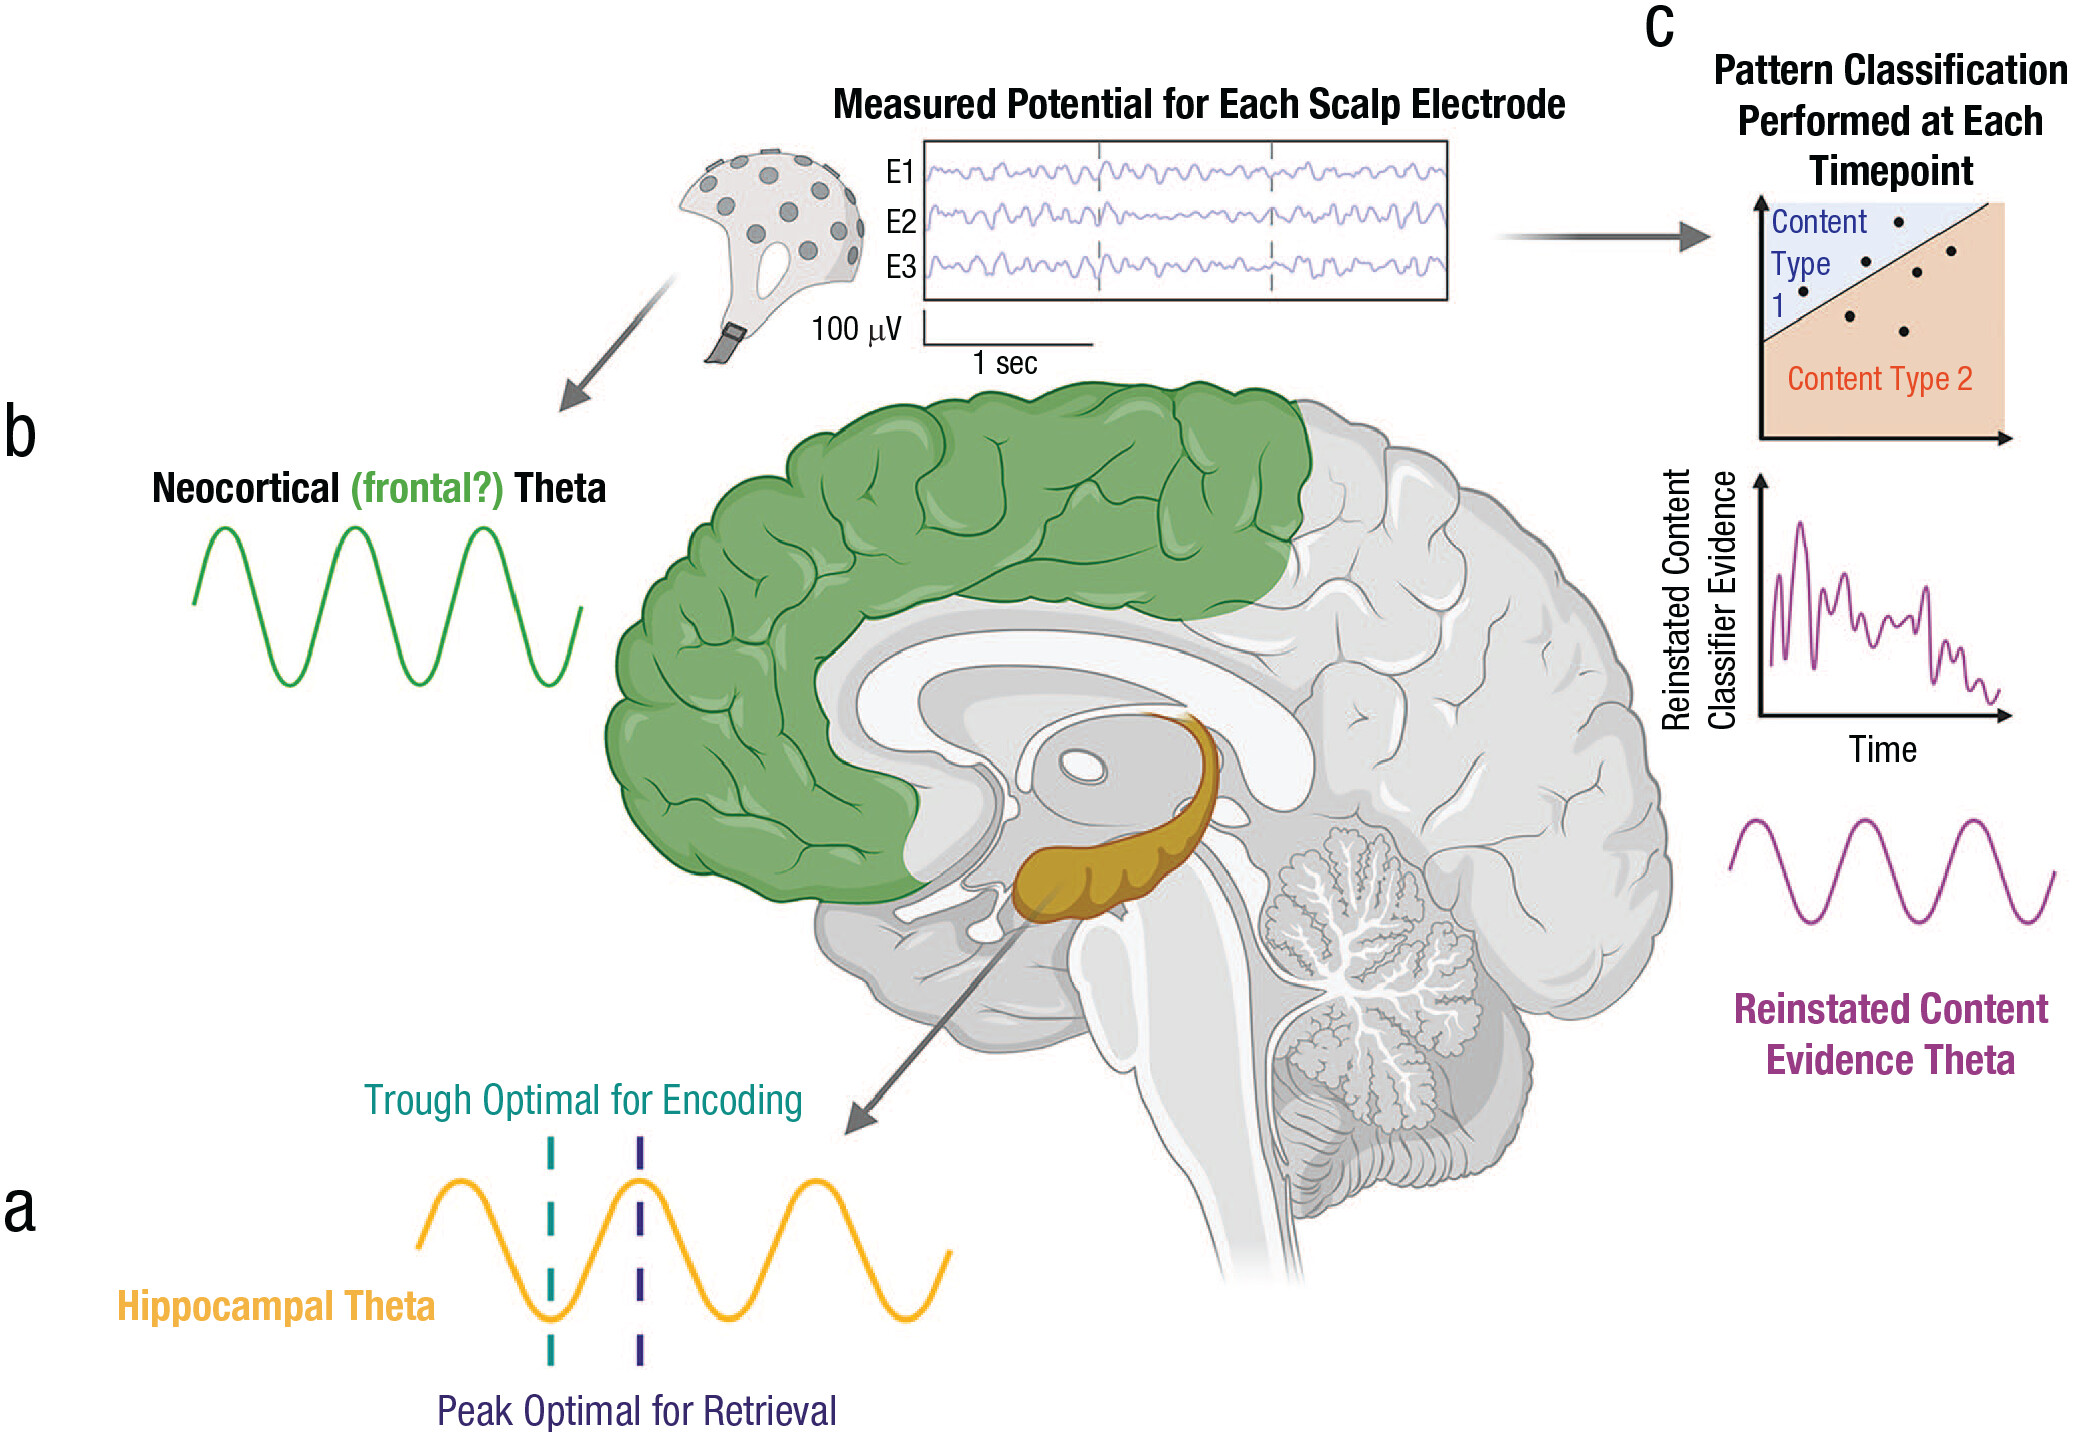
\includegraphics[width=1\linewidth]{figures/attending_to_remember-fig2.jpg}
	\caption[Three types of modeled or observed neural theta oscillations]{Three types of modeled or observed neural theta oscillations. The schematic shows (a) the SPEAR model of hippocampal theta, (b) neocortical theta power (which may or may not relate to theta oscillations in the frontoparietal cortex and/or hippocampus), and (c) theta-specific oscillations in reinstated (i.e., retrieved) episodic content (as quantified by pattern-classifier evidence in neural data). SPEAR = separate phases of encoding and retrieval. Created in BioRender \parencite{xue2025rhythmic}. \url{https://BioRender.com/p71c406}.}
	\label{fig:a2r-fig2}
\end{figure}
\FloatBarrier

Importantly, although the hippocampal theta phase \parencite{saintamour2023gamma} has been linked with encoding and retrieval success, direct evidence for the coupling of specific hippocampal phases with behavioral rhythmicity remains limited. Furthermore, there may exist encoding and retrieval modes with effects that persist over seconds \parencite{duncan2012memory}; how these prolonged mnemonic modes relate to subsecond theta-specific oscillations in hippocampal computations and behavior remains an open question. Given the nascent literature on rhythms of memory, such behavioral oscillations could be linked, at least in part, to rhythms in attention \parencite{biba2024memory}. Moreover, neural substrates of behavioral rhythms in memory may reside in the hippocampus and/or in frontoparietal attention networks.

Separately, an extensive amount of research demonstrates that theta power is linked to episodic memory functions \parencite{hsieh2014frontal,herweg2020theta}, with scalp EEG showing increases in theta power during successful encoding and retrieval (Fig.~\ref{fig:a2r-fig2}b) and intracranial EEG data from the human hippocampus and neocortex showing similar effects during associative recall \parencite{herweg2020theta,maoz2023dynamic}. Recent findings also document how the hippocampus and neocortex interact during encoding and retrieval \parencite{fernandez2024encoding,theves2024pattern,zhao2024content}, which invites questions regarding the impact of hippocampal theta oscillations on cortical representations \parencite{hanslmayr2024oscillatory}. Emerging evidence from scalp EEG suggests that the strength of encoded and retrieved event content in the neocortex, read out by machine-learning pattern-classification methods (Table~\ref{tab:glossary}), oscillates at a theta frequency \parencite[Fig.~\ref{fig:a2r-fig2}c;][]{kerren2018optimal}. Notably, peaks in cortical representational strength during learning and remembering may couple with opposing phases of a virtual hippocampal theta, although the relationship between scalp-recorded theta and hippocampal theta remains unclear \parencite{herweg2020theta,mitchell2008frontal}.

Given the uncertainty about whether oscillations of event-content representations in the neocortex relate to hippocampal theta, future research should explore whether fluctuations in the strength of to-be-encoded and retrieved cortical representations have a nonhippocampal source and are governed instead by the phase of theta oscillations that support attentional sampling \parencite{busch2010spontaneous,fiebelkorn2019rhythmic}. Moreover, future research can extend recent behavioral findings that attentional and mnemonic processes fluctuate at similar frequencies to examine their possible connections through an underlying neural rhythmicity. Recent technological advances permitting closed-loop intracranial EEG recordings during ambulatory navigation \parencite{maoz2023dynamic} could be leveraged to address these open questions more directly (for more information on closed-loop approaches, see Testing the Causality of Attention for Remembering section).

\section{Memory Precision in Aging}
Aging is accompanied by changes in specific cognitive faculties, including attention and episodic memory \parencite[e.g.,][]{fortenbaugh2015sustained,hedden2004insights}. Representational quality—including event-based feature representation (Table~\ref{tab:glossary}) during the encoding of experiences and reinstatement of previously encoded representations during retrieval—is central in many theoretical accounts and empirical investigations of age-related changes in episodic memory \parencite[e.g.,][]{stark2019mnemonic,theves2024pattern,trelle2020hippocampal}. Fortunately, advances in paradigm design and analytics promise increased sensitivity in the detection of subtle memory changes. A prominent example is the measurement of memory precision, which was originally developed to examine representational quality and quantity in working memory \parencite[e.g.,][]{ma2014changing}. Unlike classic memory tasks, in which participants indicate their memory by selecting from among a few discrete categorical decisions, assays of memory precision task participants with indicating their memory for fine-grained details using more continuous response options. For instance, during learning, participants might encounter common objects, each presented in a random color sampled from 360 possible colors; then, during retrieval, the precision of memory for an object’s study-phase color is probed by having participants indicate their memory by selecting a color using a 360-degree color wheel \parencite[Fig.~\ref{fig:a2r-fig3}; e.g.,][]{sutterer2016retrieval}. This approach can be generalized to probe memory precision for any feature that can be mapped onto an approximately perceptually uniform space, such as location, orientation, or shape \parencite{cooper2019cortico,li2020validated,richter2016distinct}.

\begin{figure}[ht!]
	\centering
	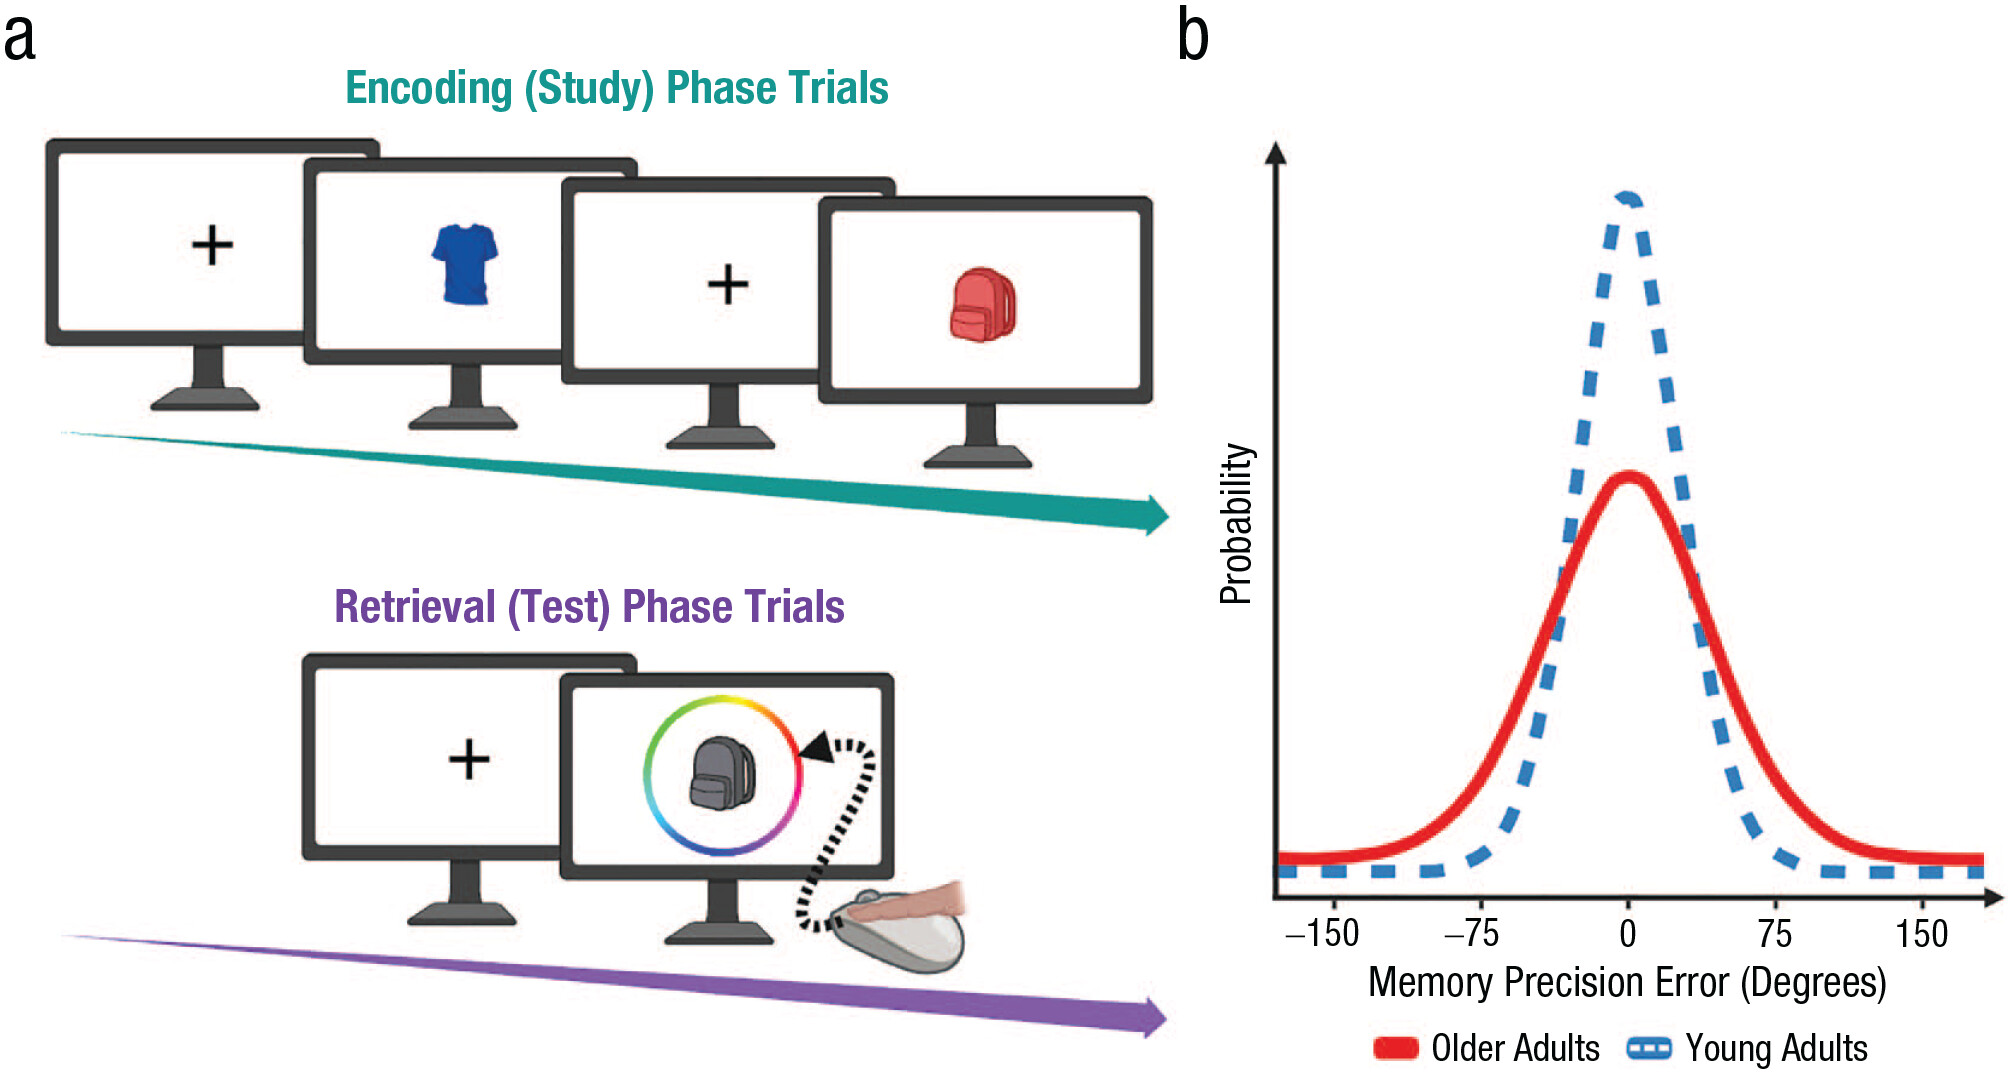
\includegraphics[width=1\linewidth]{figures/attending_to_remember-fig3.jpg}
	\caption[Example episodic memory precision task]{Example episodic memory precision task. Participants encounter (a, top) objects shaded in one of 360 possible colors. Participants then encounter (a, bottom) a grayscale version of previously encountered objects and indicate their memory for the color of the object by clicking the corresponding color on the wheel. Illustrative distributions of (b) memory precision errors are mapped from the circular space to the linear space of $-180$ to $+180$. Here, young adults (blue dashed line) are schematized to demonstrate higher memory precision than older adults (solid red line). Created in BioRender \parencite{schwartz2025b}. \url{https://BioRender.com/n00n200}.}
	\label{fig:a2r-fig3}
\end{figure}

Research on age-related episodic memory decline demonstrates the utility and promise of probing memory precision \parencite[e.g.,][]{korkki2020healthy,nilakantan2018distinguishing}. For example, \textcite{korkki2020healthy} tasked young and older participants to encode the location, color, and orientation of objects and probed subsequent memory precision for each of the three features. They fit the retrieval data with a mixture model \parencite{zhang2008discrete}, which some posit separates guesses from memory judgments varying in precision, and found that the precision estimate declined consistently with age across all three feature dimensions. \textcite{richter2016distinct} leveraged a memory precision paradigm and mixture modeling to demonstrate that different expressions of episodic memory map onto distinct neural substrates, with functional MRI activity in the hippocampus showing a categorical effect (being more active when any memory information was retrieved regardless of its precision) and activity in the angular gyrus showing a continuous effect (scaling with the precision of retrieved mnemonic features). \textcite{korkki2023reduced} replicated this relationship between episodic memory precision and angular gyrus activity and further observed that variability in precision may relate to neocortical structural variability (Table~\ref{tab:glossary}).

Notably, in \textcite{souza2024older}, older adults benefited more than young adults from a retro-cue\footnote{A retro-cue is a cue that appears after (hence, ``retro") a number of stimuli have been presented, indicating which stimulus the participant will be tested on.} directing their attention toward a particular to-be-remembered stimulus out of several others just prior to being probed about their memory for the stimulus (i.e., memory precision for the stimulus’ color). By contrast, when no retro-cue was provided (i.e., when participants did not know which of the several stimuli would be tested in the seconds after the initial stimulus array presentation), young adults outperformed older adults in terms of memory precision. Although the delay between encoding and retrieval in \textcite{souza2024older} was much shorter than that in \textcite{korkki2023reduced}, given that multiple stimuli were presented within and across memory encoding trials prior to the retrieval trials in \textcite{korkki2023reduced}, this pattern of results raises the possibility that age-related declines in memory precision may be attributed, in part, to age-related differences in selective attention.

One theory-informing application of memory precision paradigms could be to shed new light on neural dedifferentiation and its links to attention in aging \parencite[e.g.,][]{koen2020age,park2013dynamic}. Neural dedifferentiation is a prominent age-related change in the neural underpinnings of perception and episodic memory. It consists of a reduction in the selectivity of cortical activity with age, is posited to decrease the fidelity (or precision) of memory representations, and may, in part, result from declines in attention. Indeed, recent findings indicate that, in cognitively unimpaired older adults, age-related declines in memory are explained, in part, by two independent pathways: a decline in memory-related encoding activity in the dorsal attention network that in turn accounts for declines in neural selectivity, and the presence of preclinical Alzheimer’s disease pathology (as evidenced by plasma pTau181) that separately accounts for declines in neural selectivity \parencite{sheng2024top}. A test of this account of dedifferentiation could come from integrating memory precision assays with measures of neural representational precision and readouts of attention (e.g., from pupillometry and/or EEG); doing so promises to deepen understanding of the multiple drivers of neurocognitive aging.

\section{Testing the Causality of Attention for Remembering}
Historically, attempts to investigate the causal relationship between attention and memory have relied on manipulations in which a participant’s attention is divided across a primary and secondary task \parencite[e.g.,][]{baddeley1984attention,craik1996effects,murdock1965effects} or in which two feature dimensions—one relevant and one irrelevant on any given trial—compete for attention \parencite[e.g.,][]{uncapher2009selecting}. This experimental approach has yielded a rich literature revealing worse memory performance when attention is divided versus when fully focused on memory-relevant information.

In this article, much of our discussion has centered on correlational observations of attention-memory interactions. Such findings, although informative, do not permit causal inferences. Over the last few decades, advances in computing and closed-loop interfaces (Table~\ref{tab:glossary}) have enabled a complementary approach to bridging this gap \parencite[Fig.~\ref{fig:a2r-fig4}a; e.g.,][]{debettencourt2015closed,debettencourt2018forgetting,debettencourt2019realtime,keene2022pupillometry,salari2016dissociation,yoo2012when}. To illustrate, \textcite{debettencourt2019realtime} examined how attentional states impact working memory using a real-time adaptive approach. Through moment-to-moment sampling of response time on a sustained attention task, \textcite{debettencourt2019realtime} tracked intrinsic fluctuations of attention, detecting when a participant was in exceptionally high- or low-attention states. In turn, they delivered working memory probes during these optimal and suboptimal attention states\footnote{Note that these attentional states fluctuate on a longer timescale (seconds) than the theta/alpha rhythms (tens or hundreds of milliseconds) referenced in the Rhythmic Nature of Attention and Memory section; the difference in temporal frequency of these states underscores the possibility of nested attentional dynamics operating concurrently to influence memory and other cognitive behaviors.} and observed superior performance in the former. Notably, this closed-loop approach generally affords greater control over factors of interest along with increased power.

Adaptive experimental approaches can be extended to causal investigations of episodic memory-attention interactions (Fig.~\ref{fig:a2r-fig4}a). Using a real-time framework, one (or multiple concurrent) psychophysiological readouts of fluctuations in sustained attention \parencite[e.g., via pupillometry; see][]{keene2022pupillometry} could control either the temporal delivery of events to optimal versus suboptimal moments or trigger salient reorienting cues to reengage attention during momentary lapses just prior to engaging in the act of encoding or retrieval (Figs.~\ref{fig:a2r-fig4}b and \ref{fig:a2r-fig4}c). However, despite the advantages afforded by closed-loop approaches for more precise causal investigations, unforeseen challenges may arise when designing such experiments. When developing a closed-loop pipeline, researchers should adhere to signal processing best practices/limitations, rigorous testing of computational/hardware integration and implementation, and A/B testing the efficacy of intervention parameters before deploying an experiment at large. That said, these tradeoffs permit an innovative and powerful approach for causal investigations of attention’s impacts on subsequent cognitive behavior, advancing understanding of the multiple processes that collectively influence whether and how we learn and remember experiences.

\begin{figure}[!tbp]
	\centering
	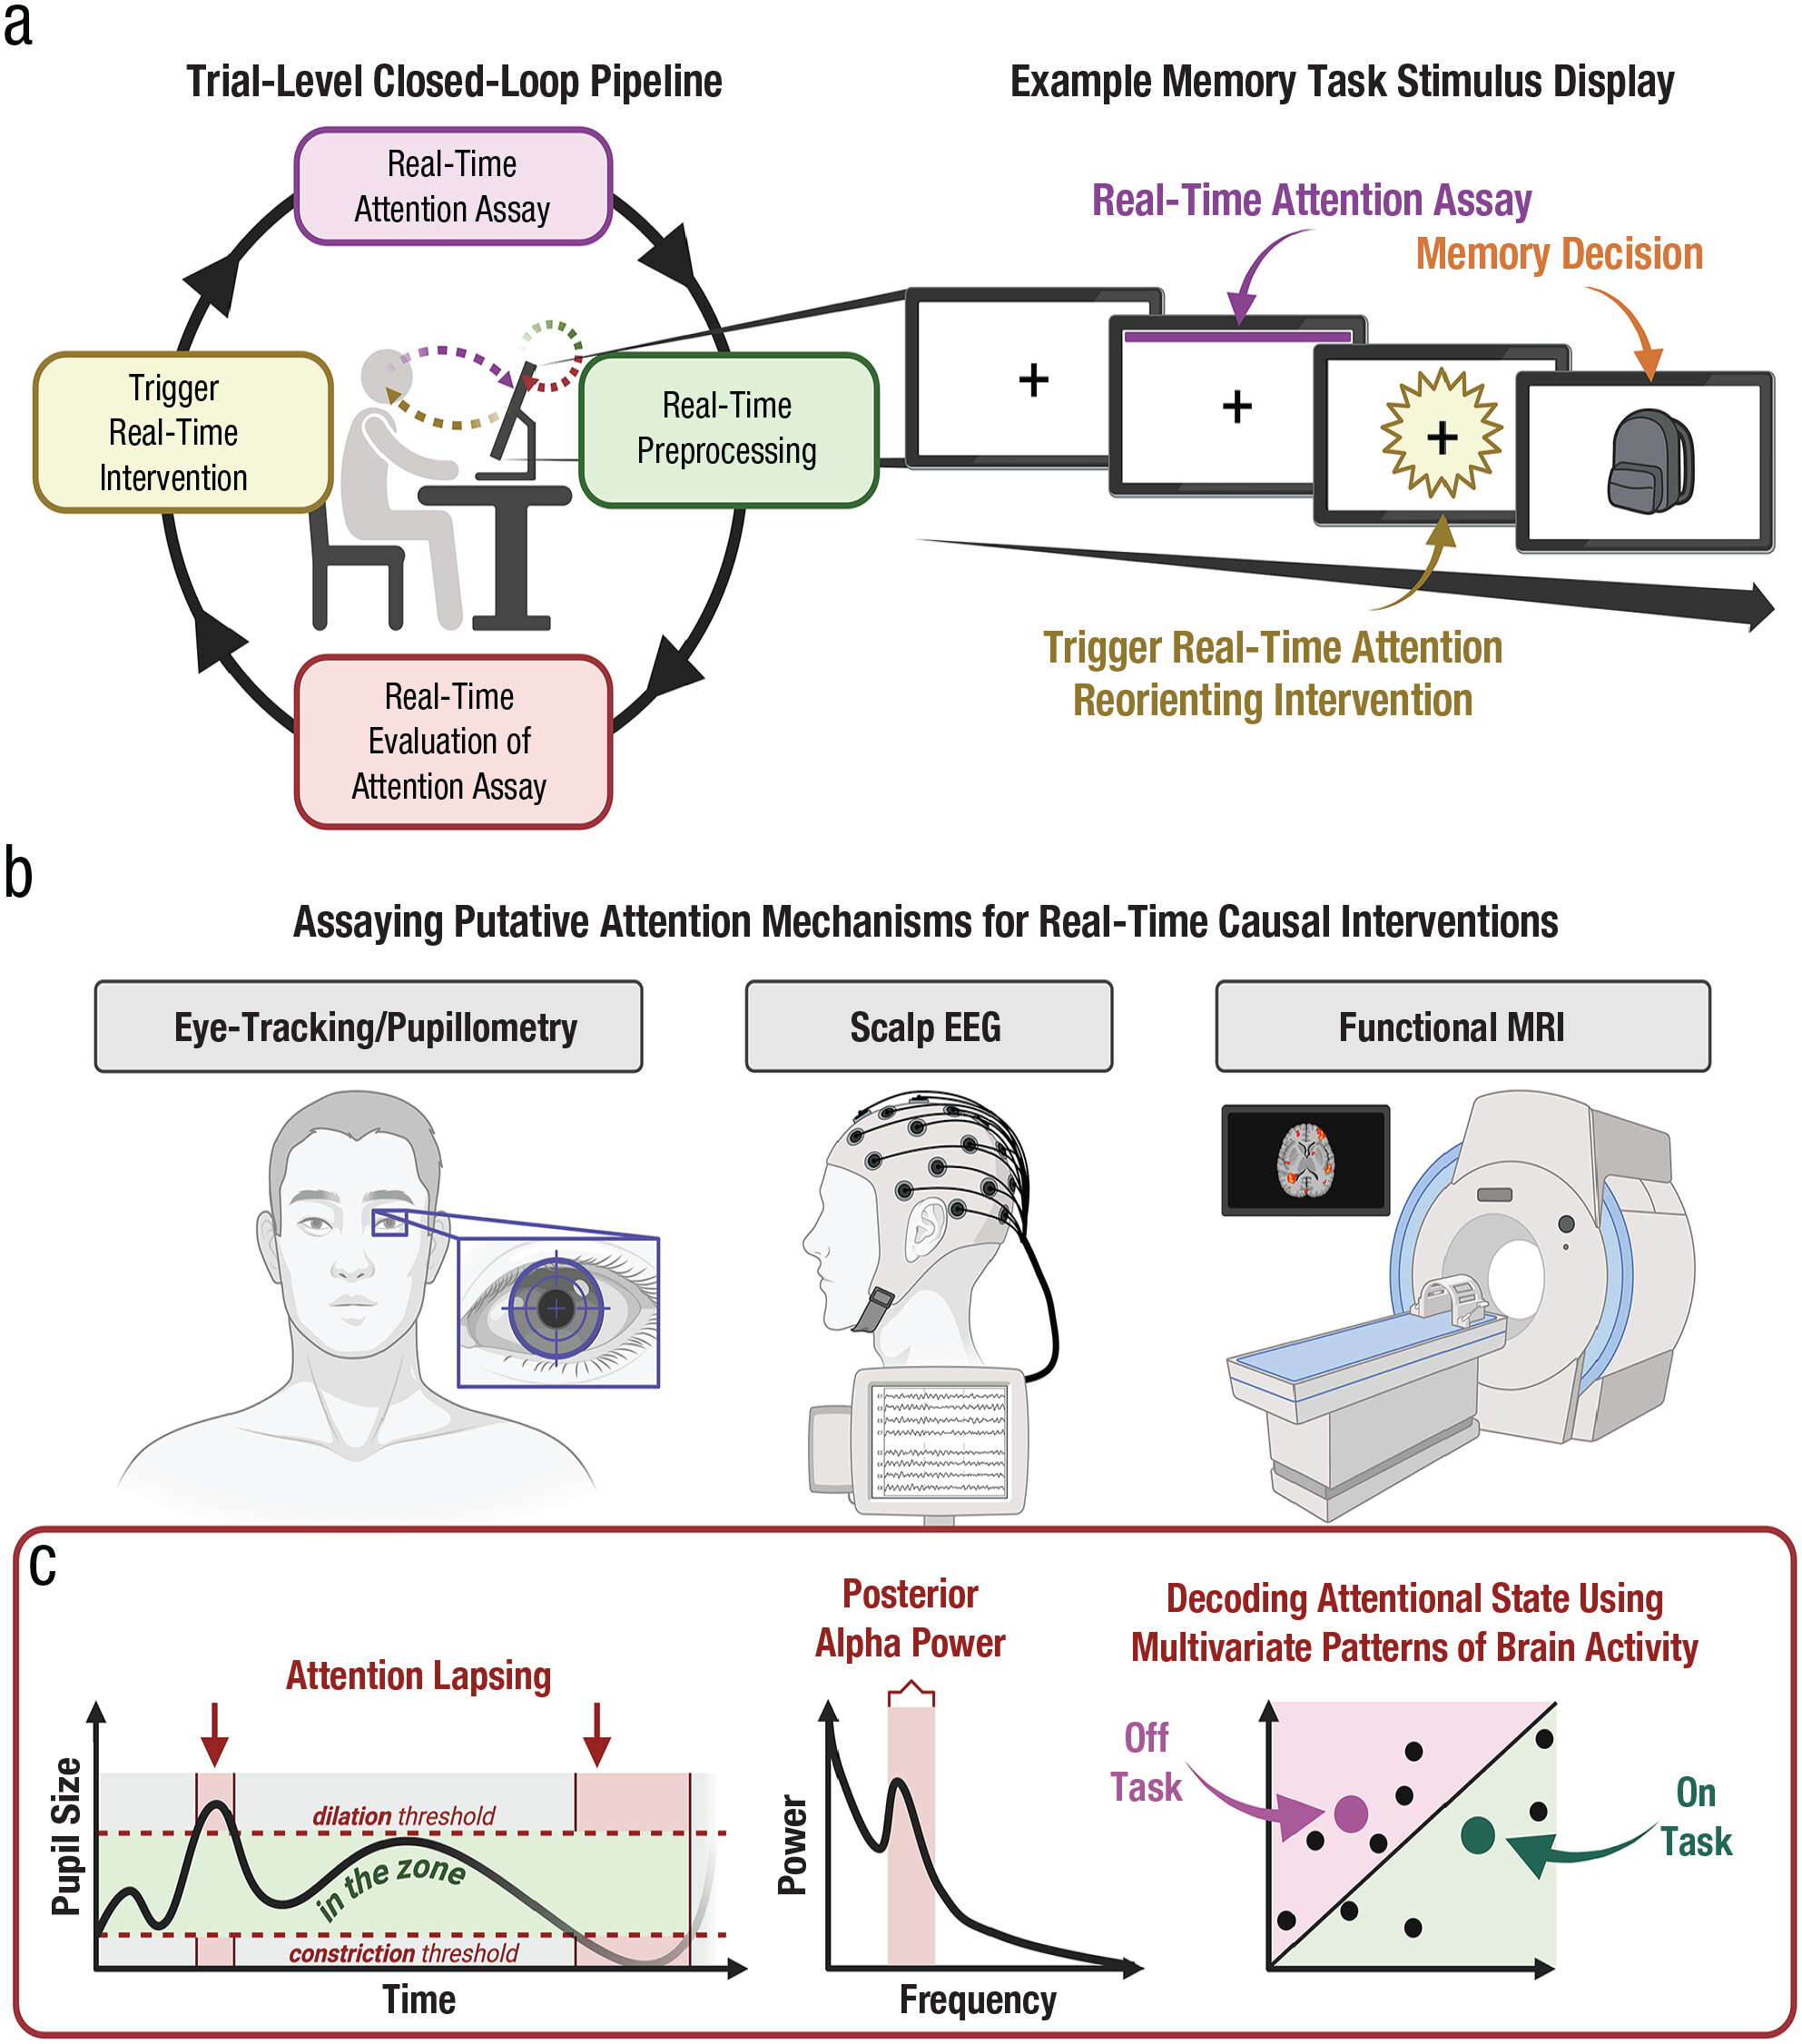
\includegraphics[width=1\linewidth]{figures/attending_to_remember-fig4.jpg}
	\caption[Innovative techniques for real-time closed-loop interventions on attention (and cognition more broadly)]{Innovative techniques for real-time closed-loop interventions on attention (and cognition more broadly). Real-time causal intervention studies require constructing and validating a robust (a, left) trial-by-trial pipeline to measure, clean, evaluate, and act on psychophysiological assays in real-time, which then can be used to manipulate the stimulus display, such as that for an (a, right) adaptive memory task with real-time attention tracking and reorienting. Example approaches for the real-time evaluation of psychophysiological assays of attention include (b, left) pupillometry (c, left; e.g., pupil-size dilation or constriction that surpasses a real-time adaptive baseline pupil threshold), (b, middle) scalp EEG (c, middle; e.g., elevated posterior alpha power), and (b, right) functional MRI (c, right; e.g., pattern-classifier decoding of attentional state). Created in BioRender \parencite{schwartz2025c}. \url{https://BioRender.com/k46d189}.}
	\label{fig:a2r-fig4}
\end{figure}
\FloatBarrier

\section{Concluding Remarks}

This article highlighted some recent advances in understanding the neurocognitive mechanisms of attention, episodic memory, and their interactions. We expect that future research and further methodological developments will continue to drive theoretical progress, enabling researchers to tackle the open questions raised herein and generate increasingly precise accounts of the systems and mechanisms that enable humans to learn and remember from life events, as well as how mnemonic function changes in aging and disease.
